\documentclass[letterpaper,12pt,fleqn]{article}
\usepackage{matharticle}
\usepackage{tikz}
\pagestyle{empty}
\begin{document}
\section*{Real Analysis}
The prerequisites for the definitions and theorems of analysis are
important. For example, consider the \emph{Extreme Value Theorem}:

\begin{theorem}
If $f:[a,b]\to\mathbb{R}$ is continuous then:
\begin{enumerate}
\item $\exists\,c\in[a,b]$ such that $f(c)$ is an absolute minimum for $f$ on
$[a,b]$.
\item $\exists\, d\in[a,b]$ such that $f(d)$ is an absolute maximum for $f$ on
$[a,b]$.
\end{enumerate}
\end{theorem}

\begin{center}
\begin{tikzpicture}[scale=0.5]
\draw (0,0) -- (10,0);
\draw (1,2) to [out=-60, in=180] (3,1);
\draw (3,1) to [out=0, in=180] (7,4);
\draw (7,4) to [out=0, in=120] (9,3);
\draw [dashed] (1,0) -- (1,2);
\draw [dashed] (3,0) -- (3,1);
\draw [dashed] (7,0) -- (7,4);
\draw [dashed] (9,0) -- (9,3);
\draw [fill=black] (1,2) circle [radius=0.1];
\draw [fill=black] (9,3) circle [radius=0.1];
\node [below] at (1,0) {a};
\node [below] at (3,0) {c};
\node [below] at (7,0) {d};
\node [below] at (9,0) {b};
\end{tikzpicture}
\end{center}

This is ``deep'' because:
\begin{enumerate}
\item It is non-constructive.
\item It is almost false.
\end{enumerate}

\bigskip

Consider what happens when the interval is not closed:

\bigskip

\begin{tikzpicture}[scale=0.75]
\draw (0,0) -- (5,0);
\draw (1,2) to [out=-15, in=120] (4,1);
\draw [dashed] (1,0) -- (1,2);
\draw [dashed] (4,0) -- (4,1);
\draw [fill=white] (1,2) circle [radius=0.1];
\draw [fill=black] (4,1) circle [radius=0.1];
\node [below] at (1,0) {a};
\node [below] at (4,0) {b};
\node at (2.5,-1) {$(a,b]$};

\draw (7,0) -- (12,0);
\draw (8.1,-2) to [out=90, in=-90] (10.9,2);
\draw [dashed] (8,-2) -- (8,2);
\draw [dashed] (11,-2) -- (11,2);
\node [below left] at (8,0) {a};
\node [below right] at (11,0) {b};
\node at (9.5,-3) {$(a,b)$};
\end{tikzpicture}

%Note that the first graph has no maximum on the interval and the second graph
%has neither a maximum nor a minimum on the interval.

Consider what happens when the function is not continuous on the interval:

\bigskip

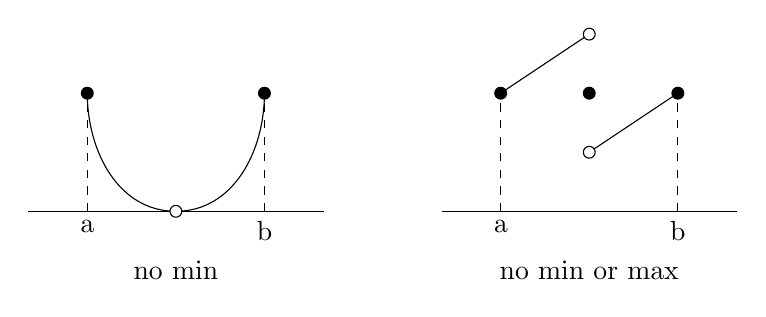
\begin{tikzpicture}[scale=0.75]
\draw (0,0) -- (5,0);
\draw (1,2) to [out=-90, in=180] (2.5,0);
\draw (2.5,0) to [out=0, in=-90] (4,2);
\draw [dashed] (1,0) -- (1,2);
\draw [dashed] (4,0) -- (4,2);
\draw [fill=black] (1,2) circle [radius=0.1];
\draw [fill=black] (4,2) circle [radius=0.1];
\draw [fill=white] (2.5,0) circle [radius=0.1];
\node [below] at (1,0) {a};
\node [below] at (4,0) {b};
\node at (2.5,-1) {no min};

\draw (7,0) -- (12,0);
\draw (8,2) -- (9.5,3);
\draw (9.5,1) -- (11,2);
\draw [dashed] (8,0) -- (8,2);
\draw [dashed] (11,0) -- (11,2);
\draw [fill=black] (8,2) circle [radius=0.1];
\draw [fill=black] (9.5,2) circle [radius=0.1];
\draw [fill=black] (11,2) circle [radius=0.1];
\draw [fill=white] (9.5,1) circle [radius=0.1];
\draw [fill=white] (9.5,3) circle [radius=0.1];
\node [below] at (8,0) {a};
\node [below] at (11,0) {b};
\node at (9.5,-1) {no min or max};
\end{tikzpicture}

\end{document}
